\documentclass[water,article,submit,pdftex,moreauthors]{Definitions/mdpi}

\graphicspath{{./fig}}

% MDPI internal commands - do not modify
\firstpage{1}
\makeatletter
\setcounter{page}{\@firstpage}
\makeatother
\pubvolume{1}
\issuenum{1}
\articlenumber{0}
\pubyear{2025}
\copyrightyear{2025}
%\externaleditor{Firstname Lastname} % More than 1 editor, please add `` and '' before the last editor name
\datereceived{ }
\daterevised{ } % Comment out if no revised date
\dateaccepted{ }
\datepublished{ }
%\datecorrected{} % For corrected papers: "Corrected: XXX" date in the original paper.
%\dateretracted{} % For retracted papers: "Retracted: XXX" date in the original paper.
\hreflink{https://doi.org/} % If needed use \linebreak
%\doinum{}
%\pdfoutput=1 % Uncommented for upload to arXiv.org
%\CorrStatement{yes}  % For updates
%\longauthorlist{yes} % For many authors that exceed the left citation part

% Add packages and commands here. The following packages are loaded in our class file: fontenc, inputenc, calc, indentfirst, fancyhdr, graphicx, epstopdf, lastpage, ifthen, float, amsmath, amssymb, lineno, setspace, enumitem, mathpazo, booktabs, titlesec, etoolbox, tabto, xcolor, colortbl, soul, multirow, microtype, tikz, totcount, changepage, attrib, upgreek, array, tabularx, pbox, ragged2e, tocloft, marginnote, marginfix, enotez, amsthm, natbib, hyperref, cleveref, scrextend, url, geometry, newfloat, caption, draftwatermark, seqsplit
% cleveref: load \crefname definitions after \begin{document}

% Please use the following mathematics environments: Theorem, Lemma, Corollary, Proposition, Characterization, Property, Problem, Example, ExamplesandDefinitions, Hypothesis, Remark, Definition, Notation, Assumption
%% For proofs, please use the proof environment (the amsthm package is loaded by the MDPI class).

% Full title of the paper (Capitalized)
\Title{A Drainage Density-Preserving River Network Delineation Algorithm}

% MDPI internal command: Title for citation in the left column
\TitleCitation{A Drainage Density-Preserving River Network Delineation Algorithm}

% Author Orchid ID: enter ID or remove command
\newcommand{\orcidauthorA}{0000-0002-5629-4795} % Add \orcidA{} behind the author's name
\newcommand{\orcidauthorB}{0000-0001-7580-9128} % Add \orcidB{} behind the author's name

% Authors, for the paper (add full first names)
\Author{Heng Yang $^{1}$\orcidA{}, Shuanglong Chen $^{2}$, and Hui Zheng $^{3,}$*\orcidB{}}

%\longauthorlist{yes}

% MDPI internal command: Authors, for metadata in PDF
\AuthorNames{Heng Yang, Shuanglong Chen and Hui Zheng}

% MDPI internal command: Authors, for citation in the left column
\AuthorCitation{Yang, H.; Chen, S.; Zheng, H.}

% Affiliations / Addresses (Add [1] after \address if there is only one affiliation.)
\address{%
  $^{1}$ \quad Science and Technology Research Institute, China Three Gorges Corporation, Beijing 100038, China; yang\_heng2@ctg.com.cn\\
  $^{2}$ \quad Baihetan Hydropower Plant, China Three Gorges Corporation, Liangshan 615421, China; chen\_shuanglong@ctg.com.cn\\
$^{3}$ \quad Institute of Atmospheric Physics, Chinese Academy of Sciences, Beijing 100029, China; hzheng\_iap@outlook.com}

% Contact information of the corresponding author
\corres{Correspondence: hzheng\_iap@outlook.com}

% Current address and/or shared authorship
% \firstnote{These authors contributed equally to this work and should be considered co-first authors.}

%\simplesumm{} % Simple summary

% Abstract (Do not insert blank lines, i.e. \\)
\abstract{Accurate representation of drainage density in river network delineation is crucial for hydrodynamic simulations, but existing digital elevation model (DEM)-based methods fail to preserve observed drainage density across the entire network. This study introduces a fundamentally improved DEM-based river network delineation method that preserves observed drainage density by incorporating a novel concept of upstream accumulation length, which integrates flow direction and drainage density. A test case demonstrated the method’s compatibility with widely used critical drainage area-based methods, producing identical results when using the same drainage density. The method was then applied to the Chinese Mainland using the MERIT-Hydro flow direction dataset and a drainage density dataset from the Third National Land Resources Survey of China. The resulting dataset shows superior performance in capturing drainage density variations, particularly in regions with complex topography, compared to existing datasets. The method is promising for delineating more accurate river networks by combining satellite-derived or surveyed drainage density with DEMs, thereby laying a valuable foundation for large-domain hydrodynamic simulations in vast regions of the globe that lack manually maintained river geometry datasets.}

% Keywords
\keyword{river network delineation; digital elevation model; drainage density; river geomorphology}

\begin{document}

\section{Introduction}
\label{sec:intro}

Accurate river network delineation is essential for hydrodynamic simulations. Among the various characteristics of river networks, drainage density is particularly significant \citep{mutzner2013WRR}. Drainage density is defined as the total length of river segments per unit area \citep{horton1932ETAGU, horton1945GSAB}. It serves as a key indicator of the hydrological characteristics of a region \citep{tarboton1992G}. In regions with high drainage density, water is drained more efficiently from the landscape, leading to more rapid hydrologic responses and potentially higher flood risks \citep{singh2021WRR, pallard2009HESS}. This characteristic also influences sediment transport, as more developed river networks can more effectively carry sediment \citep{tarboton1992G}.

The delineation of river networks has traditionally relied on two major approaches: digital elevation models (DEMs)-based methods \citep{tarboton1991HP, lin2021SD, yamazaki2019WRR, amatulli2022ESSD, munier2022ESSD} and satellite or aerial imagery-based methods \citep{wang2021RSE}. Imagery-based methods are well-suited for identifying the presence of rivers and often offer higher spatial resolution than DEM-based methods \citep{wang2021RSE}. Imagery-derived river networks can serve as the basis for calculating drainage density. However, the extracted river networks from imagery lack information on drainage directions and connectivity between river reaches, rendering them unsuitable for hydrodynamic simulations. On the other hand, DEM-based methods provide detailed information on flow direction and preserve the critical upstream-downstream relationships necessary for hydrodynamic simulations \citep{tarboton1991HP, lin2021SD, yamazaki2019WRR}. However, DEMs alone cannot directly identify the presence of rivers. As a result, DEM-based methods often fail to accurately represent the observed drainage density across the entire river network.

Several studies have attempted to overcome the limitations of DEM-based methods in representing drainage density. Existing DEM-based methods utilize a parameter known as the critical drainage area to delineate river networks \citep{tarboton1991HP}. This parameter is defined as the minimum area required to sustain a river segment. The smaller the critical drainage area, the more river segments are delineated, and consequently, the higher the drainage density. \citet{schneider2017GRL} developed a statistical model to estimate the critical drainage area using slope, lithology, and climate. This model was calibrated to match drainage densities from reference river networks in France and Australia and was subsequently applied globally to delineate river networks from DEMs. Another approach was proposed by \citet{lin2021SD}, who introduced a method to trim river segments from networks delineated using a small critical drainage area threshold (1 km\textsuperscript{2}). The river with the smallest drainage area is trimmed first, and this process is repeated until the drainage density within a watershed matches a value derived from machine learning. However, all existing methods are performed in an ad hoc manner. Drainage density is not incorporated into the delineation process itself but is only used in the evaluation or post-processing step. As a result, none of these existing studies can effectively preserve the observed drainage density across the entire river network.

We take a fundamentally different approach to address the challenge of DEM-based delineation. Rather than improving upon the critical drainage area-based methods, we propose a new delineation method based on upstream accumulation length. Upstream accumulation length is a novel concept introduced in this study. Unlike drainage area, which is determined solely by flow direction, upstream accumulation length is determined by both flow direction and drainage density. Our proposed algorithm leverages the upstream accumulation length to preserve the observed drainage density across the entire river network.

This paper is organized as follows. Section~\ref{sec:method} details the proposed algorithm. Section~\ref{sec:results} presents two examples of the algorithm. The first example is a simple artificial case, while the second is a real-world application of delineating river networks for the Chinese Mainland using the Multi-Error-Removed Improved-Terrain Hydrography (MERIT-Hydro) flow direction dataset \citep{yamazaki2019WRR} and a kilometer-resolution drainage density dataset produced from the Third National Land Resources Survey of China \citep{zhang2024CDB}. The first example demonstrates the compatibility between the proposed method and the critical drainage area-based method, while the second example shows its effectiveness in delineating large-domain river networks. Section~\ref{sec:conclusion} concludes the paper.

\section{Methods and Materials}
\label{sec:method}

\subsection{The Algorithm}
\label{sec:algorithm}

The algorithm consists of three main steps: (1) calculation of upstream accumulation length using flow direction and drainage density, (2) calculation of drainage area using flow direction, and (3) river network delineation using flow direction, drainage area, and upstream accumulation length. While extensive rearch has been conducted on the second step (i.e., the calculation of drainage area) \citep{zhou2019FES}, we will focus on the first and third steps in this section.

\subsubsection{Upstream Accumulation Length}
\label{sec:upstream}

Upstream accumulation length is defined as the total length of river segments that are upstream of a grid cell. This concept is introduced based on the following observations: For every grid cell in a study area, within its contributing area, the upstream accumulation length is, by definition, equal to the drainage density multiplied by the drainage area. In other words, during delineation, we can grow or shrink the river network to match the upstream accumulation length in every single grid cell. If the upstream accumulation length of a grid cell equals the observed value, the drainage density within the contributing area of that grid cell must also equal the observed value. Thus, we can develop a river network delineation algorithm that preserves the observed drainage density by utilizing upstream accumulation length.

We propose a fast algorithm to calculate the upstream accumulation length, as depicted in Figure~\ref{fig:upstream}. The algorithm is inspired by the work of \citet{zhou2019FES}. We define three types of grid cells: (1) source cells, (2) intersection cells, and (3) interior cells. The number of donor cells for source cells is 0, for intersection cells is greater than 1, and for interior cells is 1. The algorithm starts from the source cells and iteratively calculates the upstream accumulation length downstream until an intersection cell is encountered. The number of donor cells for the encountered intersection cell is then decreased by 1. The algorithm continues until all source cells are processed. This algorithm is efficient because it only requires a few passes through the grid cells, resulting in O(N) time complexity.

\begin{figure}[H]
  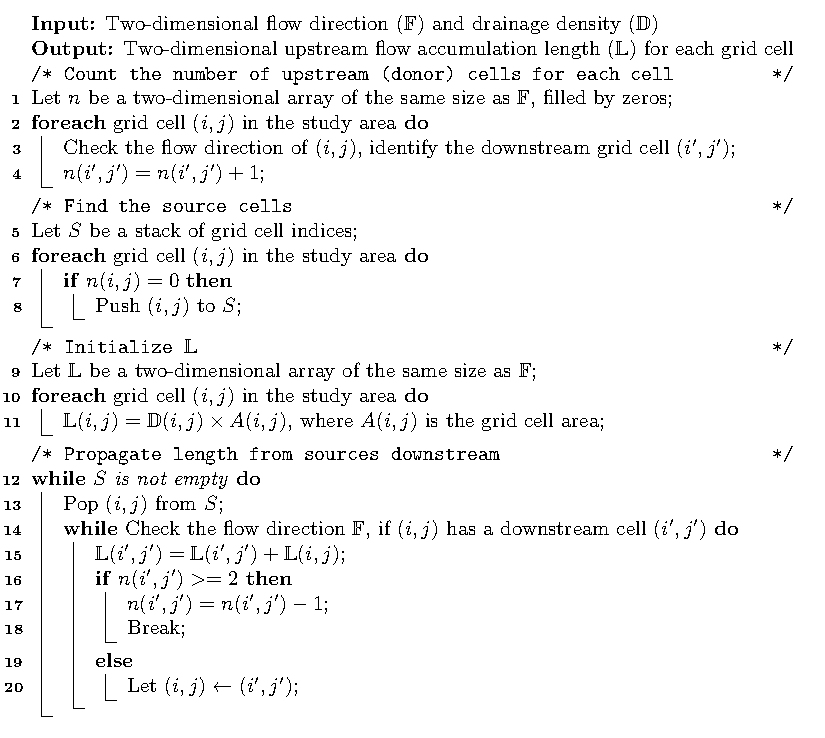
\includegraphics[width=0.9\textwidth]{upstream.pdf}
  \caption{Algorithm of calculating upstream accumulation length.\label{fig:upstream}}
\end{figure}

\subsubsection{River Network Delineation with Upstream Accumulation Length}
\label{sec:network}

As mentioned above, the objective of the delineation algorithm is to match the upstream accumulation length in every single grid cell. Numerous algorithms could be implemented to achieve this goal. In this study, we aim for our proposed algorithm to be compatible with critical drainage area-based river network delineation algorithms. We observed that in critical drainage area-based algorithms, grid cells on the delineated river network centerlines always have a larger drainage area value than those not delineated as centerlines. In other words, if one wishes to grow the river network by adding one grid cell, the grid cell with the largest drainage area among the neighbors of the delineated centerlines must be the only one considered.

Figure~\ref{fig:algorithm} details the algorithm. The algorithm starts from the outlet of the catchment and grows the river networks by adding the grid cell with the largest flow accumulation value in the neighborhood of the already delineated centerlines. The process is repeated until a bifurcating condition is encountered, which is defined as the grid cell with the largest flow accumulation value does not flow into the head grid cell of the centerline. In this case, the centerline is split into two or more sub-centerlines, which are then added to a queue for further delineation. When the length of a centerline is greater than or equal to an expected length, the delineation of the centerline stops. The expected length for a head water centerline (the one having no upstreams) is set to the upstream accumulation length of the most downstream grid cell of the centerline. The expected length for the others (the one having upstreams) are set to the upstream accumulation length of the most downstream grid cell minus the sum of the upstream accumulation length of its upstreams. With this divide-and-conquer strategy, the algorithm ensures that the delineated river network matches the upstream accumulation length in every single grid cell.

\begin{figure}[H]
  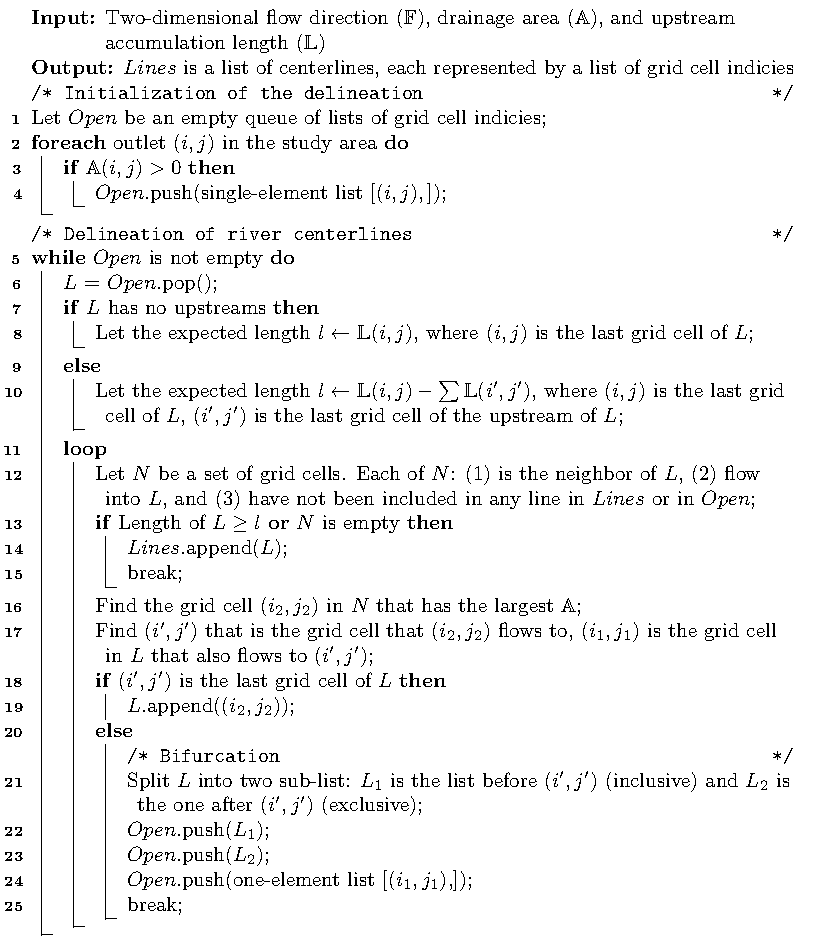
\includegraphics[width=\textwidth]{algorithm.pdf}
  \caption{Density-preserving river network delineation algorithm.\label{fig:algorithm}}
\end{figure}

\subsection{Avoidance Of Short River Segments}
\label{sec:short}

The algorithm shown in Figure~\ref{fig:algorithm} strictly preserves the observed drainage density across the entire river network. However, the algorithm often produces a large number of short river segments. These short river segments are not only difficult to represent in hydrodynamic simulations but also have a negligible impact on the overall drainage density. Figure~\ref{fig:algorithm_improve} shows an improved algorithm tailored for hydrodynamic simulations. Two thresholds are introduced in the algorithm: one for the minimum length of river segments ($l_\mathrm{cr}$, line 24 in Figure~\ref{fig:algorithm_improve}) and the other for the minimum drainage area ($A_\mathrm{cr}$, line 17 in Figure~\ref{fig:algorithm_improve}). The former is used to avoid overly short river segments on mainstreams, while the latter is used to avoid overly short river segments on head waters.

\begin{figure}[H]
  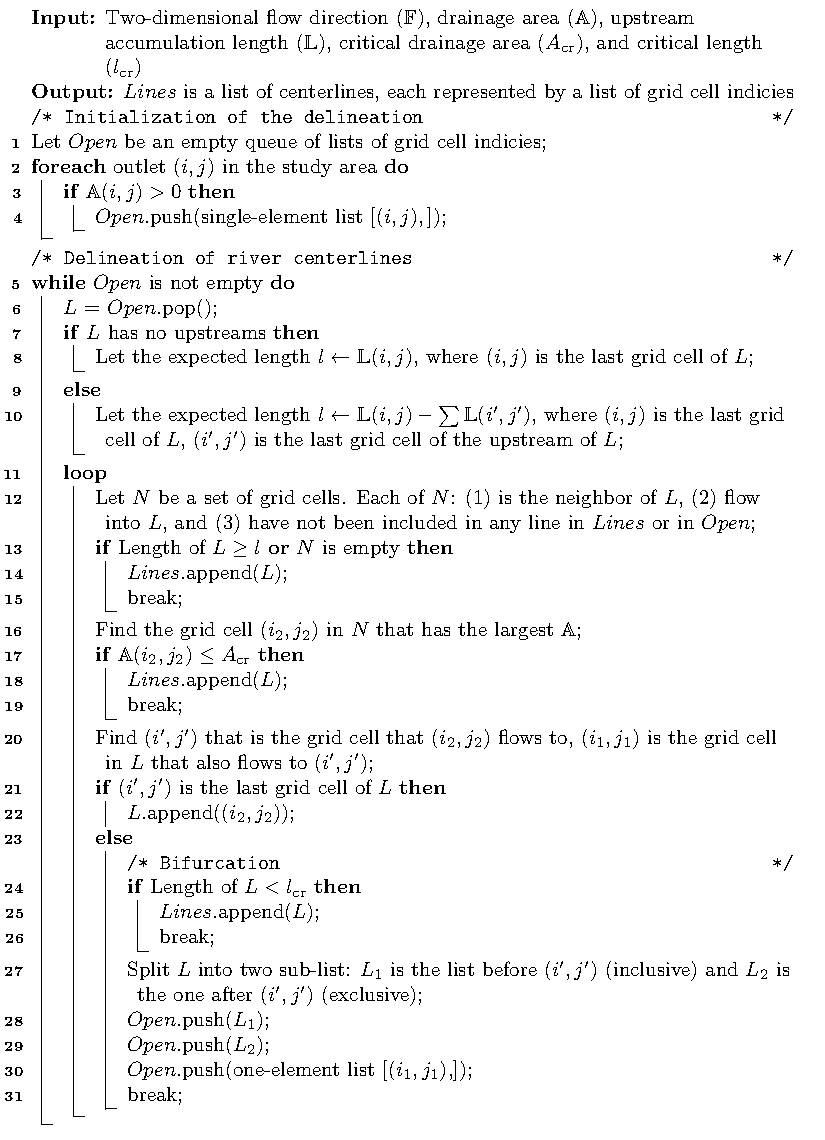
\includegraphics[width=\textwidth]{algorithm_improve.pdf}
  \caption{Density-preserving river network delineation algorithm with thresholds for river segment length and drainage area.\label{fig:algorithm_improve}}
\end{figure}

\subsection{Dataset Of Flow Direction And Drainage Density}

This study includes a real-world application of our proposed algorithm to delineate river networks over large domains. The MERIT-Hydro flow direction dataset \citep{yamazaki2019WRR} is used in this application. MERIT-Hydro is a global 3-arc-second (approximately 90 m) resolution dataset derived from the MERIT DEM \citep{yamazaki2017GRL}. This dataset has been widely used in hydrodynamic simulations \citep{yang2021BAMS}. \citet{lin2021SD} have shown that the river network delineated from the MERIT-Hydro flow direction dataset has high accuracy in terms of centerline position. Since our algorithm is compatible with critical drainage area-based algorithms, we expect that the river network delineated in this study will also achieve the same level of centerline position accuracy as reported by \citet{lin2021SD}.

We used the drainage density dataset produced from the Third National Land Resources Survey of China \citep{zhang2024CDB}. The dataset covers the entire Chinese Mainland at a spatial resolution of 1 km. The total river length within each one-kilometer grid cell is derived from the surveyed data. We bilinearly interpolated the 1-km drainage density data to the 90-m MERIT-Hydro grid.

Our study area is the Chinese Mainland, with a slightly extended boundary to ensure that the river network is continuous. The delineation is performed on the 90-m MERIT-Hydro grid. In areas without surveyed drainage density data, the drainage density is estimated using a river network delineated from the MERIT-Hydro dataset and the critical drainage area-based method with a threshold of 1 km\textsubscript{2}.

\section{Results}
\label{sec:results}

In this section, we first illustrate the algorithm using a simple example. This example is designed to demonstrate the basic steps of the algorithm and to show its compatibility with the critical drainage area-based algorithm. We then present the results of the river network delineation over the Chinese Mainland. These results are compared with those obtained using the MERIT-Hydro dataset and the critical drainage area-based algorithm. The real-world application showcases the effectiveness of the proposed algorithm in delineating river networks over large domains.

\subsection{A Simple Test Case}
\label{sec:test_case}

Figure~\ref{fig:example} illustrates the example. Figure~\ref{fig:example}a shows the flow direction of a 4$\times$4 grid. Drainage area is presented by Figure~\ref{fig:example}b, assuming that the grid size is 1$\times$1. The bottom two grid cells, which are not shown, are excluded from the following analyses for simplicity. Figure~\ref{fig:example}c presents the river centerlines delineated using drainage area with a critical drainage area threshold of 4.

Figure~\ref{fig:example}d shows the drainage density calculated from Figure~\ref{fig:example}c. Note that the river length at each grid cell is calculated as the total length of the river segments connecting the grid cell center to the centers of its upstream cells. This calculation differs slightly from survey data or imagery-based data. However, if the grid cell is small (i.e., a typical grid cell is smaller than 100 m\texttimes{}100 m), the difference is negligible. Figure~\ref{fig:example}e shows the total upstream river length calculated according to the algorithm described in Figure~\ref{fig:upstream}.

The last row of Figure~\ref{fig:example} reveals the delineation process. Figure~\ref{fig:example}f shows the state after initialization. The $Open$ queue contains the grid cells at the outlets of the catchments. After initialization, a centerline is grown from the outlet by adding the grid cell with the largest flow accumulation value in the neighborhood of the already delineated centerlines. This process is repeated until a bifurcating condition is encountered, as shown in Figure~\ref{fig:example}g.

As the grid cell with the largest flow accumulation value (denoted by the dot connected by the dashed line) does not flow into the last grid cell of the centerline, the centerline is split into two sub-centerlines, denoted by the magenta and black lines in Figure~\ref{fig:example}h. The sub-centerlines and the grid cell with the largest flow accumulation (i.e., the green line) are then added to the $Open$ queue for further delineation. However, in this simple case, the lengths of all three centerlines are greater than or equal to the expected river length, as described in Figure~\ref{fig:algorithm}, so the algorithm terminates.

In this example, the river network delineated using our proposed algorithm (Figure~\ref{fig:example}h) is identical to the one delineated using the critical drainage area-based method (Figure~\ref{fig:example}c). This demonstrates that our proposed algorithm produces the same results as critical drainage area-based methods when using the same drainage density. The only difference is that our algorithm uses drainage density as an input, while the critical drainage area-based method does not have a priori information about the drainage density.

\begin{figure}[H]
  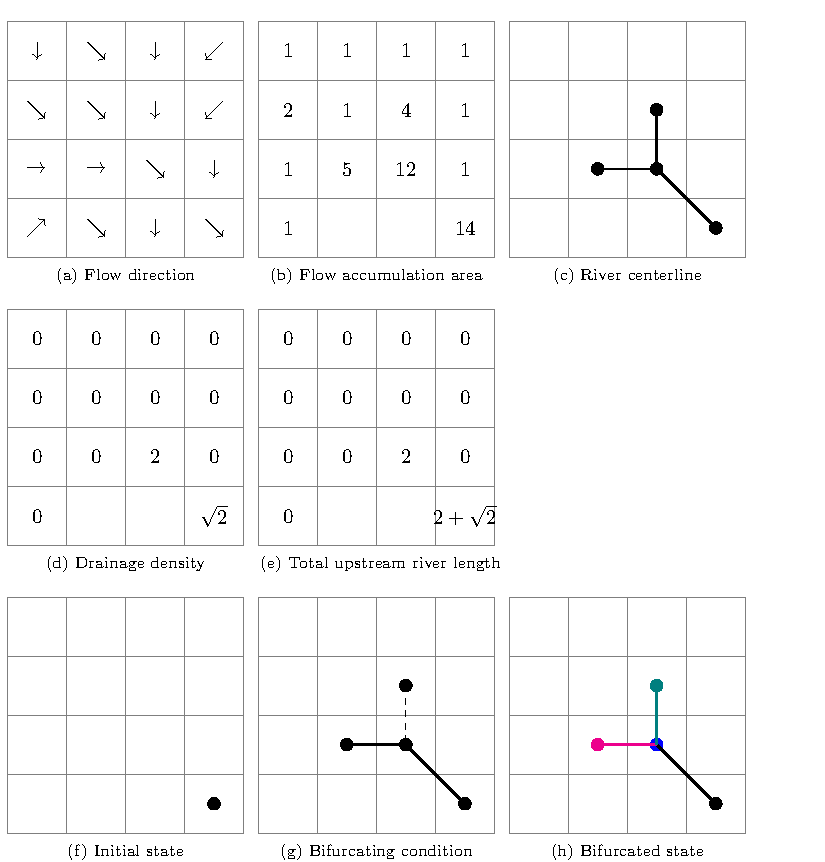
\includegraphics[width=\textwidth]{example.pdf}
  \caption{An illustration of the density-preserving river network delineation algorithm.\label{fig:example}}
\end{figure}

\subsection{A Chinese Mainland River Network Dataset For Hydrodynamic Simulations}

A river network dataset was delineated for the Chinese Mainland using the proposed algorithm. The delineation was performed on the 90-m MERIT-Hydro grid with the drainage density dataset produced from the Third National Land Resources Survey of China. The delineated river network is shown in Figure~\ref{fig:china}. The delineation was performed using the algorithm shown in Figure~\ref{fig:algorithm_improve}, with a 0.5~km\textsuperscript{2} threshold for the minimum drainage area and a 0.5~km threshold for the minimum river segment length. The delineation was performed using a single thread on a personal computer, which did not require the substantial computational resources reported in previous studies \citep{lin2021SD}. This highlights the efficiency of our proposed algorithm. The delineated river network is available at \url{https://doi.org/10.57760/sciencedb.23487} (accessed on 2024-04-10).

\begin{figure}[H]
  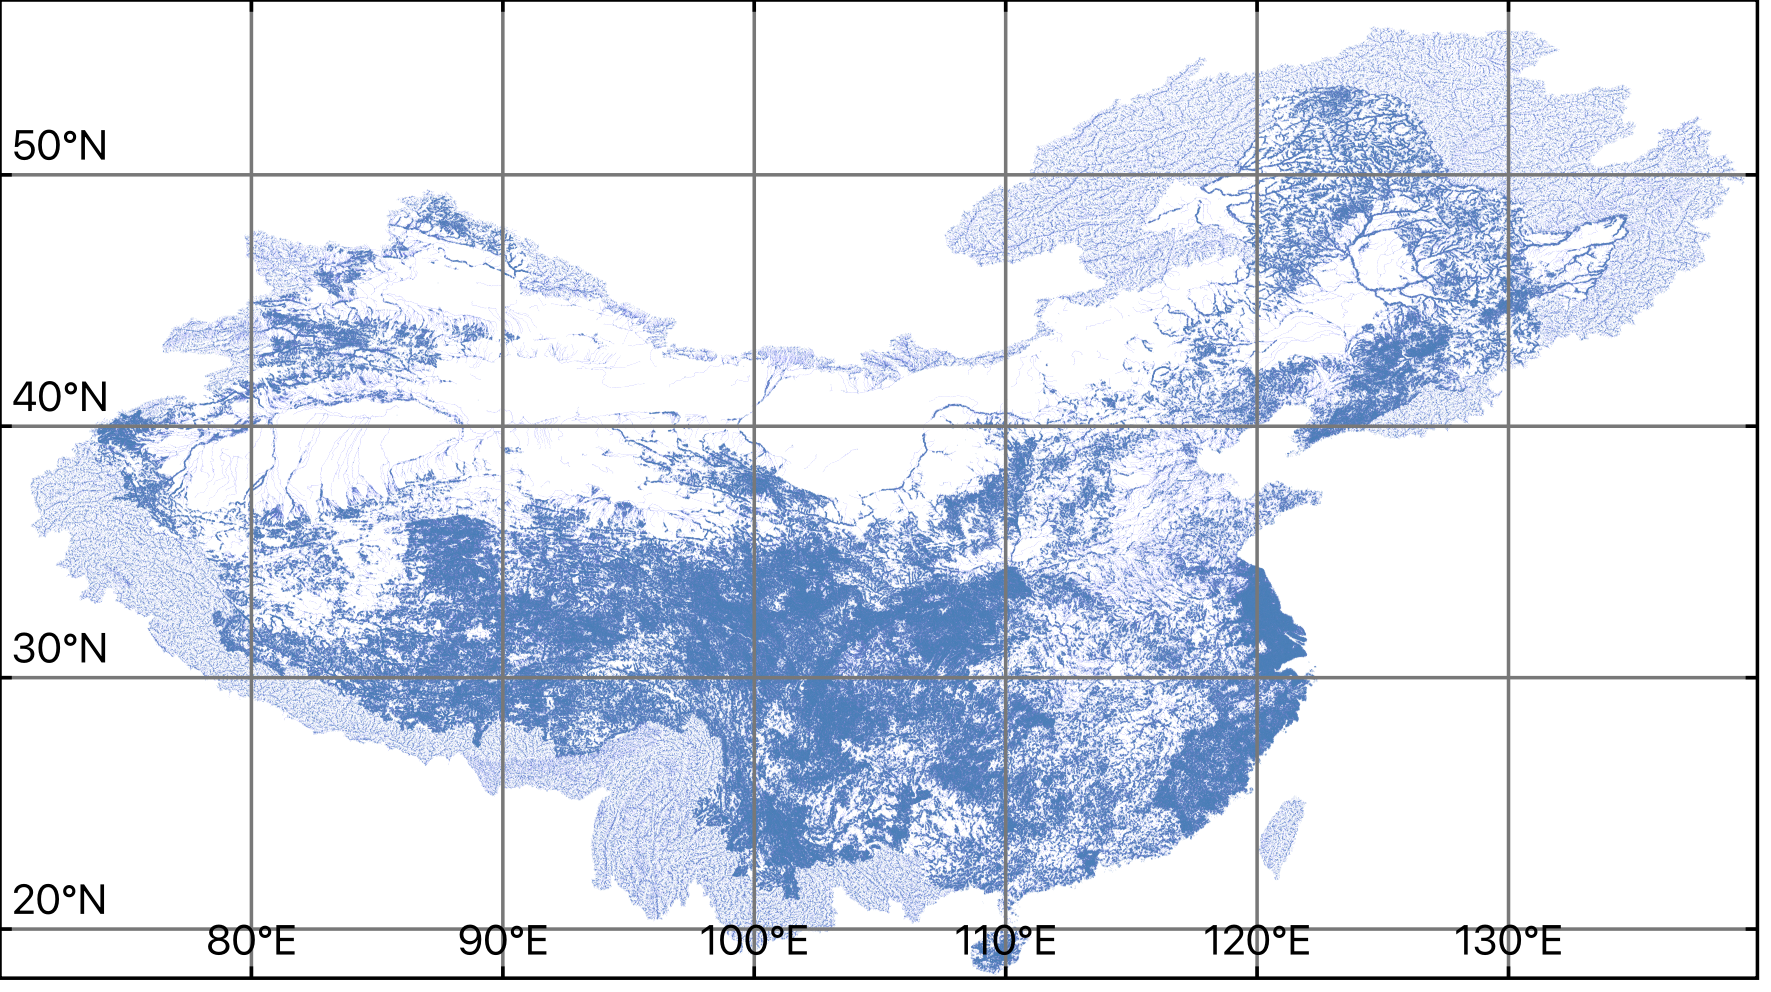
\includegraphics[width=\textwidth]{china.png}
  \caption{A Chinese Mainland river network dataset delineated using the drainage density-preserving method.\label{fig:china}}
\end{figure}

In this study, we have not evaluated the position accuracy of the delineated river network centerline. Since we are using the same flow direction dataset as \citet{lin2021SD}, we expect that the river network delineated in this study will also achieve a similar level of centerline position accuracy as reported by \citet{lin2021SD}.

Figure~\ref{fig:comparison} compares the river network delineation results in the South Xinjiang, China. South Xinjiang is characterized by a variety of landscapes, including mountains and deserts. The drainage density varies significantly across the region, making it an ideal testbed for intercomparison. Figure~\ref{fig:comparison}a shows the river network delineated using the critical drainage area-based method with a threshold of 10 km\textsuperscript{2}. The river network appears nearly uniform across the region, failing to capture the variation in drainage density. Compared with satellite imagery, the river network is overly dense in the desert areas. Figure~\ref{fig:comparison}b shows the river network delineated using the drainage density-preserving method. The result is encouraging, not only representing the contrast in drainage density between the foothills and deserts, but also resolving rivers that flow across the desert. Figure~\ref{fig:comparison}c shows the hydrological data and maps based on the Shuttle Elevation Derivatives at Multiple Scales (HydroSHEDS) river network dataset, while Figure~\ref{fig:comparison}d shows the MERIT-Vector river network dataset \citep{lin2021SD}. MERIT-Vector has a much denser network than HydroSHEDS and shows more variation in drainage density. However, they both produce overly dense river networks in the desert and show smaller variations between foothills and desert than Figure~\ref{fig:comparison}b. The comparison demonstrates that our proposed algorithm can effectively capture the variation in drainage density across the entire river network, a feature that existing publicly available datasets have not performed as well in.

\begin{figure}[H]
  %\isPreprints{} % If the paper is ``preprints'', please uncomment this parenthesis.
    \subfloat[\centering 10 km\textsuperscript{2} drainage area threshold]{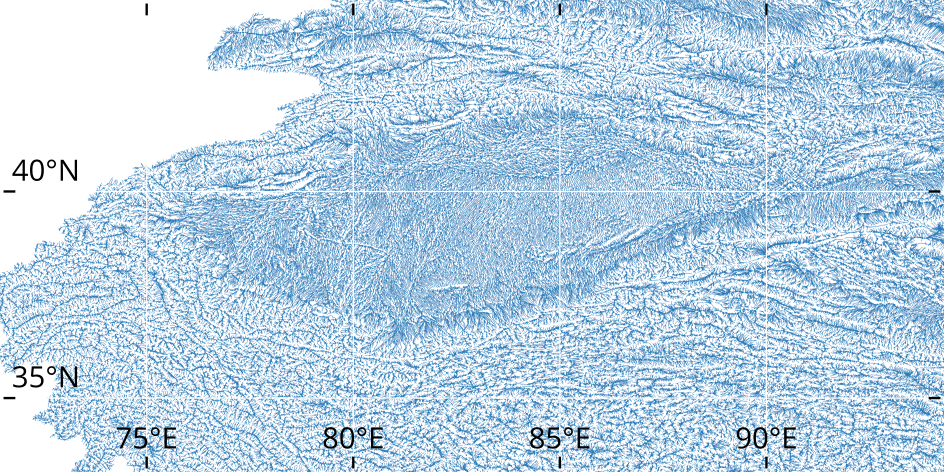
\includegraphics[width=8.0cm]{xinjiang-10km2.png}}
    %\hfill
    \subfloat[\centering The Drainage Density-Preserving Method]{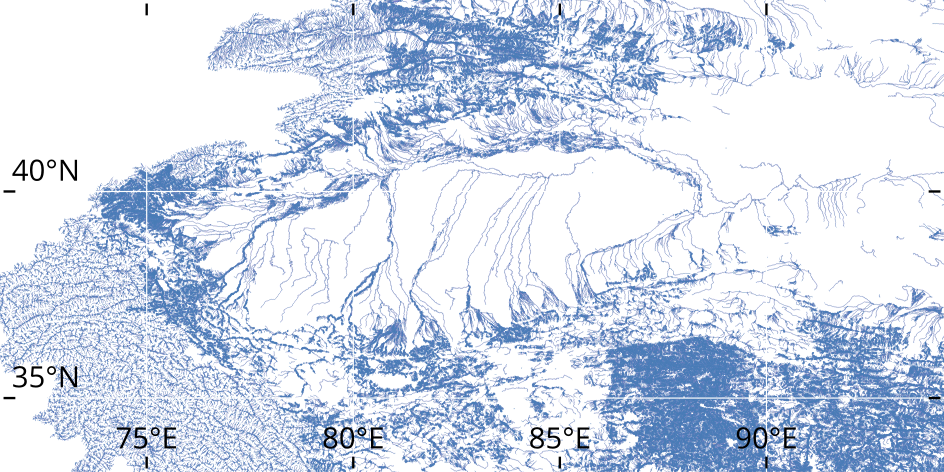
\includegraphics[width=8.0cm]{xinjiang-thisalgorithm.png}}\\
    \subfloat[\centering HydroSHEDS]{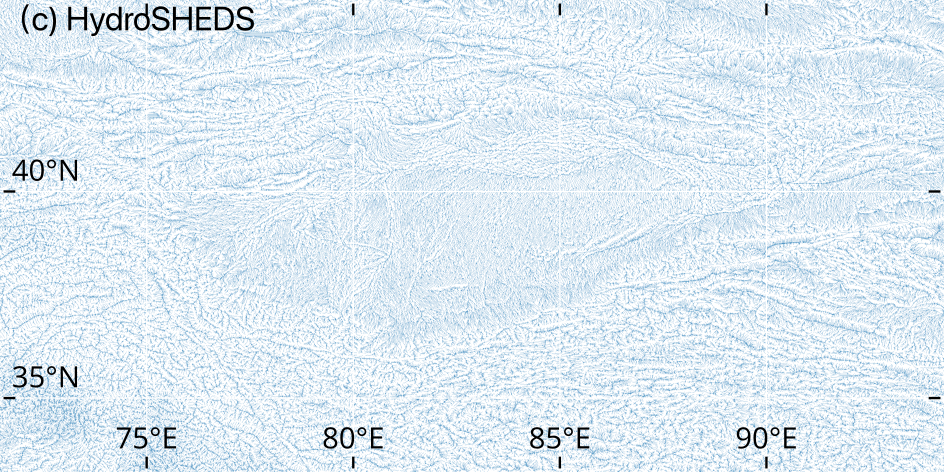
\includegraphics[width=8.0cm]{xinjiang-hydroshed.png}}
    %\hfill
    \subfloat[\centering MERIT-Vector]{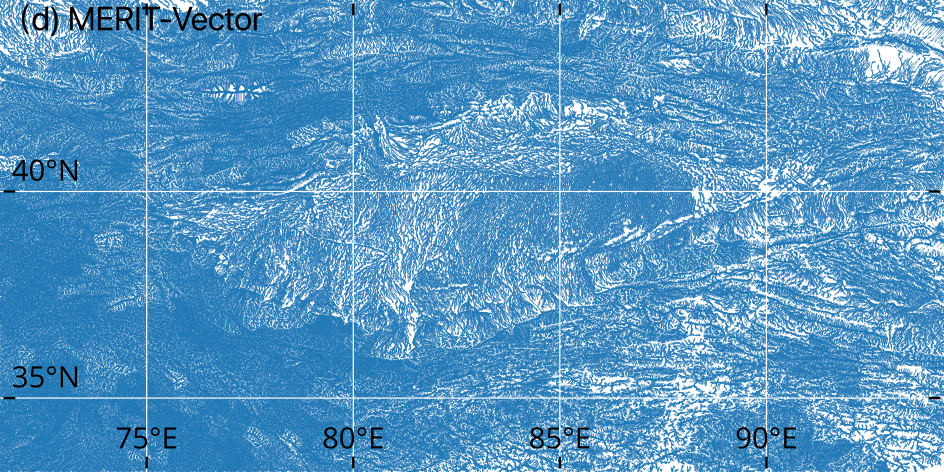
\includegraphics[width=8.0cm]{xinjiang-meritvector.png}}\\
    \subfloat[\centering Satellite Imagery]{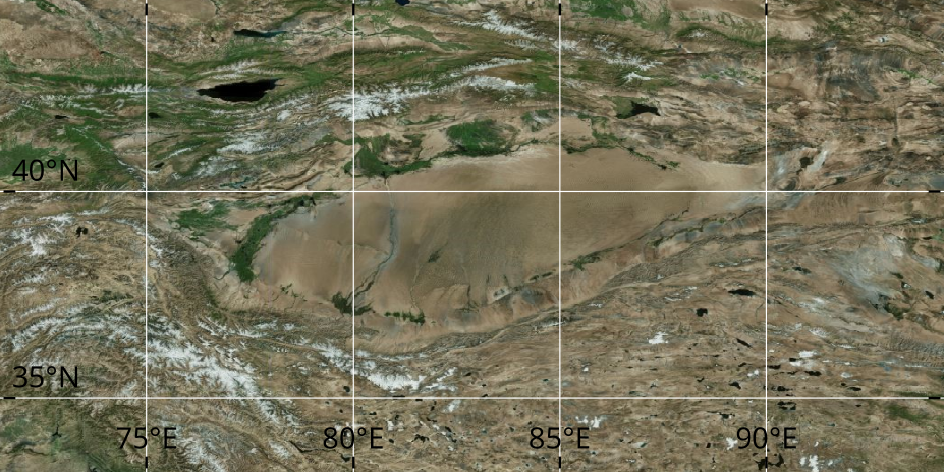
\includegraphics[width=7.0cm]{xinjiang-satellite.png}}
    %\isPreprints{}{% This command is only used for ``preprints''.
  \end{adjustwidth}
  \caption{Comparison of the river network delineation results in South Xinjiang. (\textbf{a}) delineation with critical drainage area of 10 km\textsuperscript{2}, (\textbf{b}) delineation with the drainage density-preserving method, (\textbf{c}) the HydroSHED river network dataset, (\textbf{d}) the MERIT-Vector river network dataset, and (\textbf{e}) Satellite imagery.\label{fig:comparison}}
\end{figure}

\section{Conclusions}
\label{sec:conclusion}

This study introduces a novel river network delineation method that preserves observed drainage density across the entire river network. The method is based on a novel concept named upstream accumulation length, which is calculated using flow direction and drainage density. The delineation algorithm is designed to be compatible with critical drainage area-based methods, allowing for the preservation of observed drainage density in every single catchment of the river network. The proposed algorithm was applied to the Chinese Mainland, utilizing the MERIT-Hydro flow direction dataset and a kilometer-resolution drainage density dataset produced from the Third National Land Resources Survey of China. The resulting river network dataset is segmented into nearly uniform lengths of approximately one kilometer, providing a critical foundation for the development of national-scale flood forecasting systems in the Chinese Mainland.

The assessment shows that the river network delineated in this study performs superior in capturing the variation in drainage density across the entire river network compared to other publicly available datasets. The results are encouraging, since the method opens the possibility of combining aerial satellite imagery and DEMs to delineate river networks accurately on a global scale. This is particularly important, as only a few countries (e.g., the United States of America, the United Kingdom, France, and Australia) have manually maintained river network datasets. The vast majority of the world, including China, lacks such datasets. The proposed algorithm can be applied to delineate river networks in these regions, providing a valuable resource for hydrodynamic simulations and flood forecasting systems.

Additionally, the algorithm serves as a valuable tool for studying river geomorphology. Previously, it was straightforward to calculate drainage density when river centerlines and catchments were available. Our proposed algorithm enables the reverse calculation. By preserving observed drainage density, the algorithm allows for the delineation of centerlines and catchments of a river network. This enables studies on the relationship between drainage density and drainage area. We expect more studies to be conducted in the future to enhance our understanding of drainage density and its interactions with the surrounding environment.

\vspace{6pt}

\authorcontributions{Conceptualization, H.Z.; methodology, H.Z.; software, H.Z.; validation, S.C. and H.Y.; formal analysis, S.C. and H.Y.; investigation, S.C. and H.Y.; resources, S.C., H.Y. and H.Z.; data curation, S.C. and H.Y.; writing---original draft preparation, S.C. and H.Y.; writing---review and editing, S.C., H.Y., and H.Z.; visualization, S.C. and H.Y.; supervision, H.Z.; project administration, H.Z.; funding acquisition, H.Z. All authors have read and agreed to the published version of the manuscript.}

\funding{This study is funded by China Three Gorges Corporation (contract Z532302035), the National Key Research and Development Program of China (2023YFF0805501), and the Natural Science Foundation of China (grants 42075165 and 42275178).}

\dataavailability{The MERIT-Hydro dataset was obtained from \url{https://hydro.iis.u-tokyo.ac.jp/~yamadai/MERIT_Hydro/} (accessed on 2024-11-10). The 1\,km Drainage Density Dataset in China (2022) was obtained from \url{https://doi.org/10.57760/sciencedb.16001} (accessed on 2024-11-10). The MERIT-Vector river network dataset was obtained from \url{https://doi.org/10.6084/m9.figshare.c.5052635.v1} (accessed on 2025-01-10). The HydroSHED river network dataset was obtained from \url{https://www.hydrosheds.org} (accessed on 2025-01-10). The delineated river network dataset in this study can be found on \url{https://doi.org/10.57760/sciencedb.23487} (accessed on 2024-04-10).}

\acknowledgments{We thank for the technical support of the National Large Scientific Infrastructure ``Earth System Numerical Simulation Facility'' (\url{https://cstr.cn/31134.02.EL})}

\conflictsofinterest{Authors Heng Yang and Shuanglong Chen were employed by the China Three Gorges Corporation. The remaining author declares that the research was conducted in the absence of any commercial or financial relationships that could be construed as a potential conflict of interest.}

%\isPreprints{} % If the paper is ``preprints'', please uncomment this parenthesis.
  %\printendnotes[custom] % Un-comment to print a list of endnotes

  \reftitle{References}
  \bibliography{references.bib}

  \PublishersNote{}
  %\isPreprints{} % If the paper is ``preprints'', please uncomment this parenthesis.
\end{document}
